\documentclass{article}
\usepackage[utf8]{inputenc}
\usepackage{graphicx}
\usepackage{geometry}
\usepackage{hyperref}
\hypersetup{
    colorlinks,
    citecolor=black,
    filecolor=black,
    linkcolor=black,
    urlcolor=black
}

 \geometry{
 a4paper,
 left=30mm,
 right=30mm,
 top=30mm,
 }

\graphicspath{ {Images/} }

%----------------------------------------------------------------------------------------
%	TITLE PAGE
%----------------------------------------------------------------------------------------

\newcommand*{\titleGP}{\begingroup
		\begin{figure}[t]
			\centering
			
\includegraphics[width=350px]{UP_Logo.PNG}
		\end{figure}
\centering 
\vspace*{\baselineskip}

\rule{\textwidth}{1.6pt}\vspace*{-\baselineskip}\vspace*{2pt}
\rule{\textwidth}{0.4pt}\\[\baselineskip]

{\LARGE NavUP\\ [0.3\baselineskip] Longsword Testing Report } \\ [0.2\baselineskip]
\rule{\textwidth}{0.4pt}\vspace*{-\baselineskip}\vspace{3.2pt}
\rule{\textwidth}{1.6pt}\\[\baselineskip] %

% \scshape %
% A concise specification on the functional requirements  \\
% and use cases of NavUP \\[\baselineskip]

% \vspace*{2\baselineskip}

Compiled By \\[\baselineskip]
{\Large Lucian Sargeant - u15225560 \\ Ritesh Doolabh - u15075754 \\ Peter Boxall -  u14056136 \\ Claude Greeff - u13153740\\ Harris Leshaba - u15312144 \\ Hristian Vitrychenko - u15006442\par}

\bigskip
\bigskip

 	GitHub Repository:  
 	\href{https://github.com/Chris19951225/COS-301-Longsword-Data-Streaming}{COS 301 Team Longsword Data GitHub Repository(Phase 4)}




 

\vfill


{\scshape 2017} \\[0.3\baselineskip]
{\large TEAM LONGSWORD (DATA)}\par

\endgroup}

\begin{document}

\titleGP
\newpage
\tableofcontents

\newpage
\section{Introduction}
\begin{flushleft}
For this phase we will be testing the Data module of the BroadSword Team. We have split the testing phase according to Functional Requirements, Non-Functional Requirements and Use Cases. 
\end{flushleft}

\begin{flushleft}
Their code was primarily coded in Python and used a NSQ message processing system.
We will be testing the various cases and giving a brief description of how we tested followed by an explanation of the mark that was given to them.
\end{flushleft}


\section{Service Contracts}


\subsection{Retrieving and passing device MAC address.}
\begin{flushleft}MARK: 10\end{flushleft}
The access module sends a location request to the data module via the NSQ server,the access module has to subscribes to a topic.The main entry point of the system, query\_resolver.py, sends the mac address to the aruba server in a query to get the location of the device.
In query\_resolver.py, the handler function receives a request, it then passes the mac address to the searcher function-which will create a query to get the location for the device.
\begin{flushleft}This functional requirement was fulfilled by the Broadsword team.\end{flushleft}
\begin{figure}[ht]
  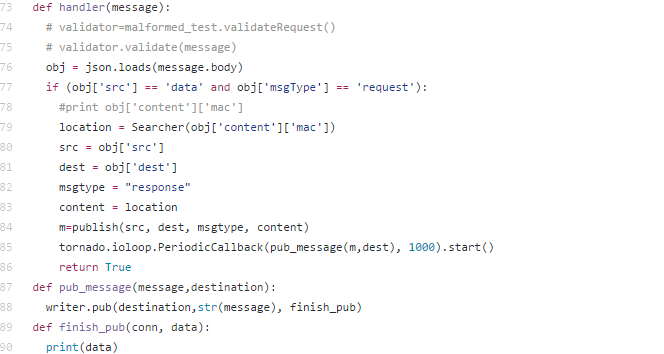
\includegraphics[width=350px]{Handler.jpg}

\caption{Handler function.}
  \label{fig:Handler function}
\end{figure}

\subsection{Logging in and maintaining a session with Aruba ALE.}


\subsection{Processing the request and retrieving location.}

\begin{flushleft}MARK: 10\end{flushleft}
In the python file query\_resolver.py, Broadsword provides the options of using mock data to test their program or to follow standard procedure and use real data from Aruba by connecting to it through location\_lookup.py, building\_lookup.py and floor\_lookup.py. The previously mentioned python files each connect to Aruba and all seperately log in by utilising aruba\_wrapper.py which establishes and maintains a session with Aruba. Each class also filters their own JSON objects that are returned by Aruba and return only the necessary data thus fulfilling the requirement of processing requests and retrieving location.   
\begin{flushleft}This functional requirement was not fully fulfilled by the Broadsword team.\end{flushleft}
\begin{figure}[ht]
  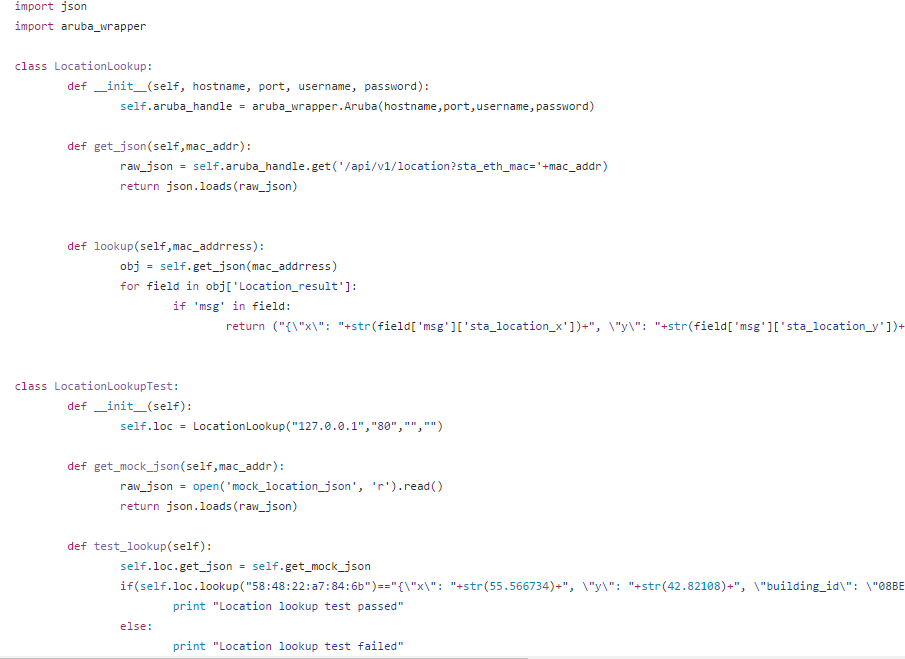
\includegraphics[width=350px]{Images/getLoc.PNG}
  \caption{aruba\_wrapper.py}
  \label{fig:aruba\_wrapper.py}
\end{figure}
\begin{figure}[ht]
  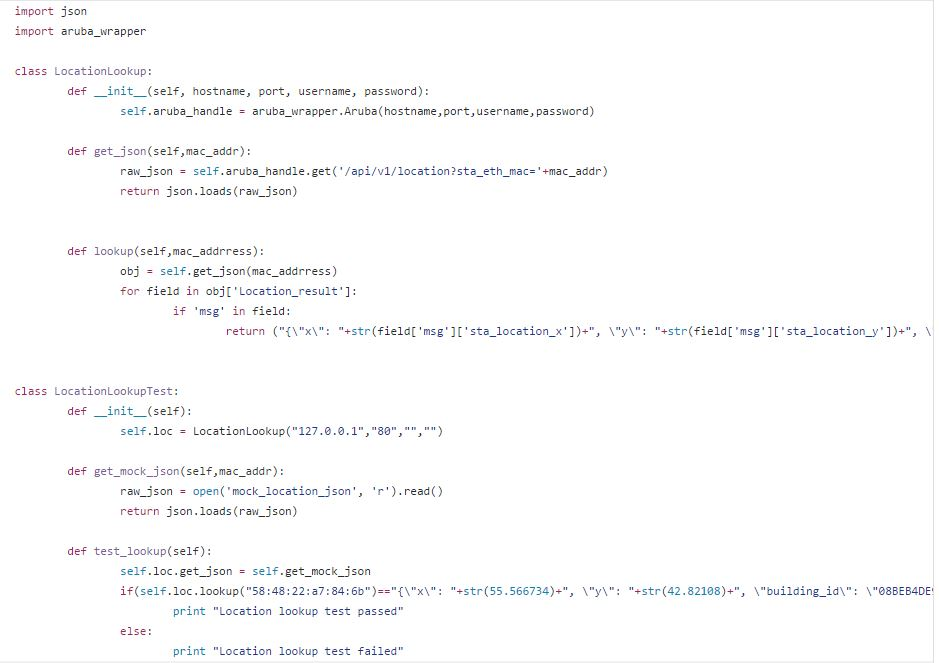
\includegraphics[width=350px]{Images/LocLookup.JPG}
  \caption{Mock JSON}

\label{Mock JSON}
\end{figure}


\subsection{Returning a location to the source of the request.}


\section{Non-Functional Requirements}

\subsection{Level of concurrency of the task.}
\begin{flushleft}MARK: 0\end{flushleft}
Broadsword made use of a server known as NSQ which is widely known for its message passing based procedures. Whilst the NSQ core was built in Go (a programming language with built in concurreny), Broadsword did not seem to make use of any of those concurrent features in their code. This was made apparent in testNavigationConsumer.py where each NSQ action was made on after the other with no concurrency apparent anywhere in terms of mac address processing and message passing. In terms of concurrent programming in general, there is a none in any of the code presented by Broadsword. 
\begin{flushleft}This non-functional requirement was not fulfilled by the Broadsword team.\end{flushleft}
\begin{figure}[ht]
  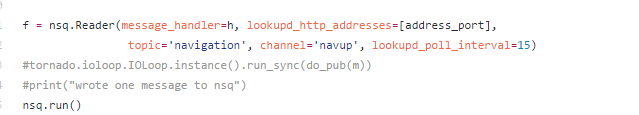
\includegraphics[width=350px]{Images/concurrency.PNG}
  \caption{NSQ Use Without Concurrency}
  \label{NSQ Use Without Concurrency}
\end{figure}
\begin{figure}[ht]
  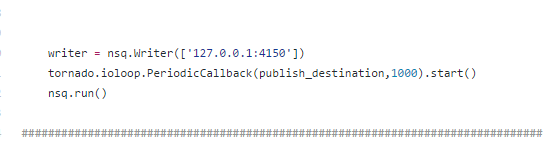
\includegraphics[width=350px]{Images/concurrency2.PNG}
  \caption{NSQ Writer}
  \label{NSQ Writer}
\end{figure}

\subsection{Performance of the request processing (time taken to receive a response).}

\subsection{Maintainability and modularity of the code and repository.}

\subsection{Integrability and ease of transfer into a final system.}


\section{Use Cases}

Broadsword has made use of a NSQ.
A 'nsqd' instance is designed to handle multiple streams of data at once.
In NSQ terms, streams are called "topics" where a topic can have 1 or more "channels".
A channel maps to a downstream service consuming a topic.
The method broadsword used was to create a topic, "data", through subscribing to channel "navup", which is a channel on the "data" topic. The topic is created through the first subscription.
This method lets channels and topics buffer their data independently. This allows for fast downstream, preventing a slow consumer to cause a bottleneck or delay.

Successful upstream and downstream communication ticks the use case boxes, although more efficient changes could be made for concurrent processing, a mark of 8 out of 10 for downstream and upstream seems fair.

\subsection{Upstream communication.}
\begin{flushleft}MARK: 8\end{flushleft}

The file named "publisher.py" will write to nsqd port 4150, this is their upstream communication channel.

\begin{figure}[ht]
  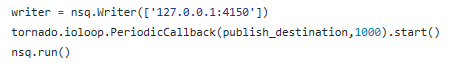
\includegraphics[width=350px]{Images/publisher.PNG}  
\end{figure}

\subsection{Downstream communication.}
\begin{flushleft}MARK: 8\end{flushleft}

Consumers make use of a HTTP /lookup endpoint. Consumers are introduced to topics through making use of the addresses of Broadsword's nsqlookupd instance. In their case it would be host name '127.0.0.1' and port '4161'. This would be their downstream communication.

\begin{figure}[ht]
  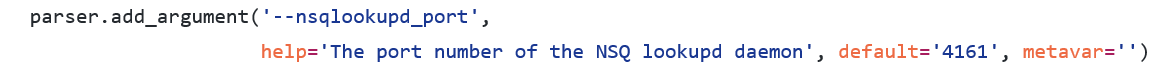
\includegraphics[width=350px]{Images/readerInitialize.PNG}  
\end{figure}

\begin{figure}[ht]
  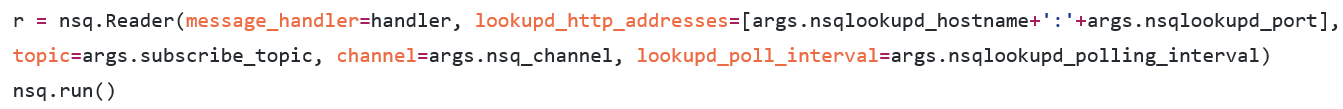
\includegraphics[width=350px]{Images/readerExecute.PNG}  
\end{figure}

\end{document}
